\chapter{Defining A Scene}

In this chapter we first see how to lay out different objects into a virtual
world, i.e. a scene.
To do this, we introduce the concept of entity.
At the end, we set up and render a simple scene to show in practice the
concepts we have described in this chapter.

\begin{figure}[ht]
    \centering
    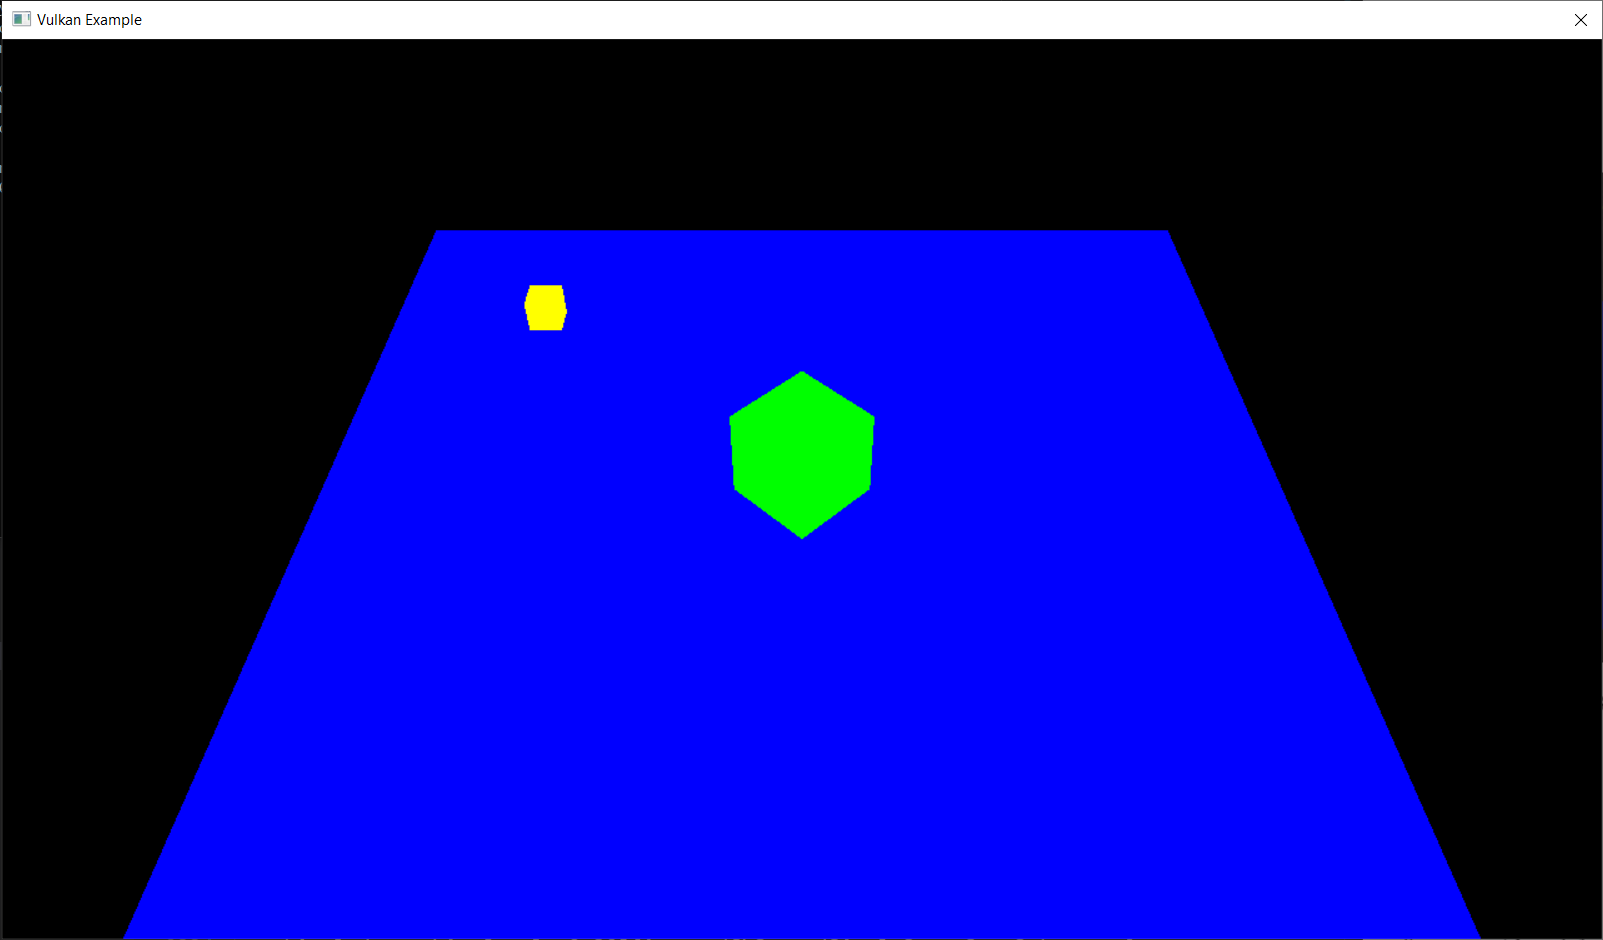
\includegraphics[scale=0.20]{images/ChScene/SimpleScene.png}
    \caption{Define and render a simple scene}
    \label{fig::SimpleScene}
\end{figure}

\section{Why Do We Need Entities?}

Suppose we want to render two squares like we did here \ref{fig::DepthTesting}.
We could, for example, use the following vertex data.

\begin{minipage}{\linewidth}{\noindent}
    \lstinputlisting[
        language=C++,
        caption={Vertices for drawing two squares},
        label={lst::TwoQuadsVertexData}
        ]{src/ChScene/TwoQuadsVertexData.cpp}
\end{minipage}

This is what we have done in all previous chapters.
We have rendered our objects directly using their vertex positions.
Although this works, it's obviously not a flexible solution.

Those of you with a keen eye have surely noticed
that our squares almost have the same vertices.
The only difference being in the $z$ coordinates.
Drawing two squares means drawing two instances of the same geometric data.
Why would we need to repeat the same data twice, just with some slight variations?
There is no reason to do it.
We can use matrices to define the transformations we want to apply to each object.
For one square we could use a matrix that doesn't apply any transformation.
For the other square we could use a matrix that translates the vertices upwards.

There is a catch.
Now, our objects are not simply defined by their vertex data.
They also have a position, a rotation, etc.
They can also share the same vertex data to avoid redundancy.
We use the concept of entity to solve this situation.

\section{Entity}

An entity is simply a collection of all the data that is necessary to place
an object in the scene and draw it accordingly.

\subsection{Entity Positional Data}

We now have an idea of the nature of entities.
We can start by defining all the data necessary
to place an entity into a scene.

Let's start with an example
We can have a cube placed at $(0, 0, 0)$, the origin of our scene.
We could place another cube at $(5, 3, 0)$ and rotate it by $30$
degrees around the $x$ axis and by $60$ degrees around the $z$ axis.
We could also place another cube around the scene and scale it by a factor
of $10$ to make it bigger than the other cubes.

From this example, we can see that our entities have three main properties
that define how the entity is contextualized inside a scene:
\begin{itemize}
    \item a 3d vector that represents its position inside the scene
    \item a 3d vector that represents its rotations around the $x, y$ and $z$ axis
    \item a scalar that represents its scale
\end{itemize}

TODO: add entity uml

\subsection{Entity Rendering Data}

In our previous example, we have talked about placing cubes around a scene.
Earlier we have discussed that entities should share their vertex data if possible.
We do this to avoid redundancy.
If two or more entities are cubes, they are fine sharing the same vertex data.
Thus, entities not only hold positional data, but also refer to some vertex data,
in our case, a vertex buffer.
We know that a vertex buffer is used in tandem with a pipeline state object for
drawing operations.
Hence, an entity should also refer to such object.

To transform our vertices from local space to world space, we use a model matrix.
We also have to use a both a view and projection matrix to transform our vertex
positions into normalized device coordinates.
These three matrices are passed to the vertex shader as uniforms through a
uniform buffer.
Hence, our entity should refer to a uniform buffer.

Contrary to the other rendering resources, we must create such uniform
buffer on an entity by entity basis.
This is because the entity's uniform data refer to the entity itself.

TODO: add entity uml

\subsection{Entity Data}

TODO: add entity uml

\section{Camera}

Our entities have a view matrix and a projection matrix as uniforms.
But from where do we get these matrices?
We get them from a camera.

TODO: go on with this reasoning

\section{Setting Up A Simple Scene}

TODO: show blender view of our scene
